%% Please change the file name by replacing N with the apporpriate number
%% corresponding to the current homework and XX with your initials.
%% https://www.math.uci.edu/~gpatrick/jsOnline/hw1.html

\documentclass{beamer}
\usepackage{amssymb,amsfonts,color,graphicx,amsmath,enumerate,mathtools}
\usepackage{tikz} %This package offers the ability to draw pictures
\usepackage{amsthm}
\usepackage{hyperref}
\usepackage{algorithm}
\usepackage[noend]{algpseudocode}

\newcommand{\naturals}{\mathbb{N}}
\newcommand{\integers}{\mathbb{Z}}
\newcommand{\complex}{\mathbb{C}}
\newcommand{\reals}{\mathbb{R}}
\newcommand{\exreals}{\overline{\mathbb{R}}}
\newcommand{\mcal}[1]{\mathcal{#1}}
\newcommand{\mable}{measurable}
\newcommand{\quats}{\mathbb{H}}
\newcommand{\rationals}{\mathbb{Q}}
\newcommand{\norm}{\trianglelefteq}
\newcommand{\Aut}{\text{Aut}}
\newcommand{\disk}{\mathbb{D}}
\newcommand{\halfplane}{\mathbb{H}}
\newcommand{\Lp}[2]{\left\|{#1}\right\|_{L^{#2}}}
\newcommand{\supp}[1]{\text{supp}({#1})}
\newcommand{\Hom}[2]{\text{Hom}_{{#1}}({#2})}
\newcommand{\tr}{\text{tr}}
\newcommand{\field}[1]{\mathbb{F}_{{#1}}}
\newcommand{\Gal}[1]{\text{Gal}\left({#1}\right)}
\newcommand{\esssup}{\text{ess sup }}
\newcommand{\essinf}{\text{ess inf }}
\newcommand{\affine}{\mathbb{A}}
\DeclareMathOperator*{\argmin}{arg\,min}

\newtheorem{proposition}[theorem]{Proposition}

\title{The LLL Algorithm}
\author{Liam Hardiman}
\usetheme{Frankfurt}


% Roadmap
% Motivation
%	good basis, bad basis
% LLL
%	Gram Schmidt
%	The algorithm
%		description
%		runtime
%	return to good basis bad basis
% Coppersmith
%	improvement
%	ROCA
%  

\AtBeginSection[]{
	\begin{frame}<beamer>
		\tableofcontents[currentsection]
	\end{frame}
}


\begin{document}
\maketitle

\section{Motivation}
\begin{frame}
	\frametitle{Two lattices}
	\begin{itemize}
		\item Recall that the \textbf{lattice}, $L$, generated by the linearly independent vectors $x_1, x_2, \ldots, x_n\in \reals^n$ is the $\integers$-span of these vectors:
		\[
		L = \{c_1x_1 + c_2x_2 + \cdots + c_nx_n: c_i \in \integers, 1\leq i \leq n\}.
		\]\pause

		\item Consider the lattices, $L$ and $M$, generated by the rows of the matrices $X$ and $Y$, respectively.	
		\[
		X = \begin{bmatrix*}[r]
			-168 & 602 & 58\\
			157 & -564 & -57\\
			594 & -2134 & -219\\
		\end{bmatrix*}, \quad
		Y = \begin{bmatrix*}[r]
			-6 & 6 & -4\\
			9 & 4 & 1\\
			-1 & 8 & 6\\
		\end{bmatrix*}.
		\]
	\end{itemize}
\end{frame}

\begin{frame}
	\frametitle{Two lattices}
	\begin{itemize}
		\item Each row of $X$ is an integer linear combination of the rows of $Y$, so $L\subseteq M$:\pause
		\begin{align*}
		\begin{bmatrix*}[r]
			-168\\602\\58
		\end{bmatrix*}^T &= 14 \begin{bmatrix*}[r]
			4\\2\\-9
		\end{bmatrix*}^T + 50 \begin{bmatrix*}[r]
			-1\\8\\6
		\end{bmatrix*}^T -29 \begin{bmatrix*}[r]
			6\\ -6\\ 4
		\end{bmatrix*}^T,\\	
		\begin{bmatrix*}[r]
			157\\ -564\\ -57
		\end{bmatrix*}^T &= -13 \begin{bmatrix*}[r]
			4\\2\\-9
		\end{bmatrix*}^T - 47 \begin{bmatrix*}[r]
			-1\\8\\6
		\end{bmatrix*}^T + 26 \begin{bmatrix*}[r]
			6\\-6\\4
		\end{bmatrix*}^T,\\
		\begin{bmatrix*}[r]
			594\\-2134\\-219
		\end{bmatrix*}&= -49 \begin{bmatrix*}[r]
			4\\2\\-9
		\end{bmatrix*}^T - 178 \begin{bmatrix*}[r]
			-1\\8\\6
		\end{bmatrix*} + 102 \begin{bmatrix*}[r]
			6\\-6\\4
		\end{bmatrix*}^T.
		\end{align*}
	\end{itemize}
\end{frame}

\begin{frame}
	\frametitle{Two lattices}
	\begin{itemize}
		\item In particular, we have the matrix equation\\
	\end{itemize}
	\begin{align*}
	UY&= X,\\
	\begin{bmatrix*}[r]
		14 & 50 & -29\\
		-13 & -47 & 27\\
		-49 & -178 & 102
	\end{bmatrix*}
	\begin{bmatrix*}[r]
		4 & 2 & -9\\
		-1 & 8 & -6\\
		6 & -6 & 4
	\end{bmatrix*}&=
	\begin{bmatrix*}[r]
		-168 & 602 & 58\\
		157 & -564 & -57\\
		594 & -2134 & -219
	\end{bmatrix*}.
	\end{align*}\pause

	\begin{itemize}
		\item $\det U = -1$, so $U^{-1}$ is an integer matrix as well. This gives us another matrix equation, $Y = U^{-1}X$.\pause
		\item Since the entries of $U^{-1}$ are integers, this equation expresses the rows of $Y$ as integer linear combinations of the rows of $X$, so $M\subseteq L$.
	\end{itemize}
\end{frame}

\begin{frame}
	\frametitle{Two lattices}
	\begin{itemize}
		\item Even though the rows of $X$ and $Y$ generate the same lattice, something about the $Y$-basis ``feels'' nicer.
		\[
		X = \begin{bmatrix*}[r]
			-168 & 602 & 58\\
			157 & -564 & -57\\
			594 & -2134 & -219\\
		\end{bmatrix*}, \quad
		Y = \begin{bmatrix*}[r]
			-6 & 6 & -4\\
			9 & 4 & 1\\
			-1 & 8 & 6\\
		\end{bmatrix*}.\pause
		\]
		\item Two qualities that make a basis desirable are:
		\begin{itemize}
			\item Length: how long are the basis vectors?
			\item Orthogonality: are the basis vectors nearly orthogonal to each other?
		\end{itemize}
	\end{itemize}
\end{frame}

\begin{frame}
	\frametitle{What makes a basis ``nice''?}
	\begin{itemize}
		\item Suppose $x_1, x_2, \ldots, x_n\in \reals^n$ are pairwise orthogonal.\pause
		\item If $x = c_1x_1+c_2x_2 + \cdots + c_nx_n$, $c_i\in \integers$, is in the lattice $L$ generated by $x_1, \ldots, x_n$ then
		\[
		|x|^2 = c_1^2|x_1|^2 + c_2^2|x_2|^2 + \cdots + c_n^2|x_n|^2.\pause
		\]
		\item This completely solves the shortest vector problem (SVP) since
		\[
		\argmin_{x\in L}|x| = \argmin_{x\in \{\pm x_1, \pm x_2, \ldots, \pm x_n\}}|x|.
		\]
	\end{itemize}
\end{frame}

\begin{frame}
	\frametitle{What makes a basis ``nice''?}
	\begin{itemize}
		\item Say we want to find a vector in $L$ that is closest to
		\[
		x = t_1x_1 + t_2x_2 + \cdots + t_nx_n,
		\]
		where the $t_i$ are \textit{real} numbers.\pause
		\item If $y = c_1x_1+c_2x_2 + \cdots + c_nx_n$, $c_i\in \integers$, is any vector in $L$ then by the orthogonality of the $x_i$ we have
		\[
		|x-y|^2 = (t_1-c_1)^2|x_1|^2 + (t_2-c_2)^2|x_2|^2 + \cdots + (t_n-c_n)^2|x_n|^2.\pause
		\]
		\item If we take $c_i$ to be the closest integer to $t_i$ then we solve the closest vector problem (CVP).
	\end{itemize}
\end{frame}

\begin{frame}
	\frametitle{Measuring orthogonality}
	\begin{definition}
		Let $x_1, \ldots, x_n$ be a basis for the lattice $L\subset \reals^n$. We define the determinant of $L$, $\det L$ to be the volume of the $n$-dimensional parallelepiped with sides defined by $x_1, \ldots, x_n$:
		\[
		\det L = |\det X|,
		\]
		where the rows of $X$ are the basis vectors $x_1, \ldots, x_n$.
	\end{definition}\pause
	\begin{theorem}
		The determinant of $L$ is independent of basis.
	\end{theorem}
\end{frame}

\begin{frame}
	\frametitle{Measuring Orthogonality}
	\begin{itemize}
		\item The volume of the parallelepiped defined by $x_1, \ldots, x_n$ is maximized when when the basis vectors are pairwise orthogonal to one another.\pause
		\begin{theorem}[Hadamard's Inequality]
			Let $x_1, \ldots, x_n$ be a basis for the lattice $L\subset \reals^n$. Then
			\[
			\det L\leq |x_1||x_2|\cdots |x_n|.\pause
			\]
		\end{theorem}
		\item If the basis vectors are closer to being orthogonal, then Hadamard's inequality is closer to an equality.
	\end{itemize}
\end{frame}

\section{Gram-Schmidt}
\begin{frame}
	\frametitle{Gram-Schmidt}
		\begin{definition}
			Let $x_1, \ldots, x_m \in \reals^n$ be a basis for a nonzero subspace, $H$. The \textbf{Gram-Schmidt process} produces an orthogonal basis for $H$:
			% \begin{align*}
			% 	x_1^* &= x_1\\
			% 	x_2^* &= x_2 - \frac{x_2\cdot x_1^*}{x_1^*\cdot x_1^*}x_1^*\\
			% 	x_3^* &= x_3 - \frac{x_3\cdot x_1^*}{x_1^*\cdot x_1^*}x_1^* - \frac{x_3\cdot x_2^*}{x_2^*\cdot x_2^*}x_2^*\\
			% 	\vdots\\
			% 	x_m^* &= x_m - \frac{x_m\cdot x_1^*}{x_1^*\cdot x_1^*}x_1^* - \cdots - \frac{x_m\cdot x_{m-1}^*}{x_{m-1}^*\cdot x_{m-1}^*}x_{m-1}^*.
			% \end{align*}
			\begin{align*}
				x_1^* &= x_1\\
				x_2^* &= x_2 - \mu_{2, 1}x_1^*\\
				x_3^* &= x_3 - \mu_{3,1}x_1^* - \mu_{3,2}x_2^*\\
				\vdots\\
				x_m^* &= x_m - \mu_{m,1}x_1^* - \cdots - \mu_{m, m-1}x_{m-1}^*,
			\end{align*}
			where $\mu_{i,j} = \frac{x_i\cdot x_j^*}{x_j^*\cdot x_j^*}$. We call $\{x_1^*, \ldots, x_m^*\}$ the \textbf{Gram-Schmidt orthogonalization (GSO)} of $\{x_1, \ldots, x_m\}$.
		\end{definition}
\end{frame}

\begin{frame}
	\frametitle{Gram-Schmidt}
	\begin{figure}
	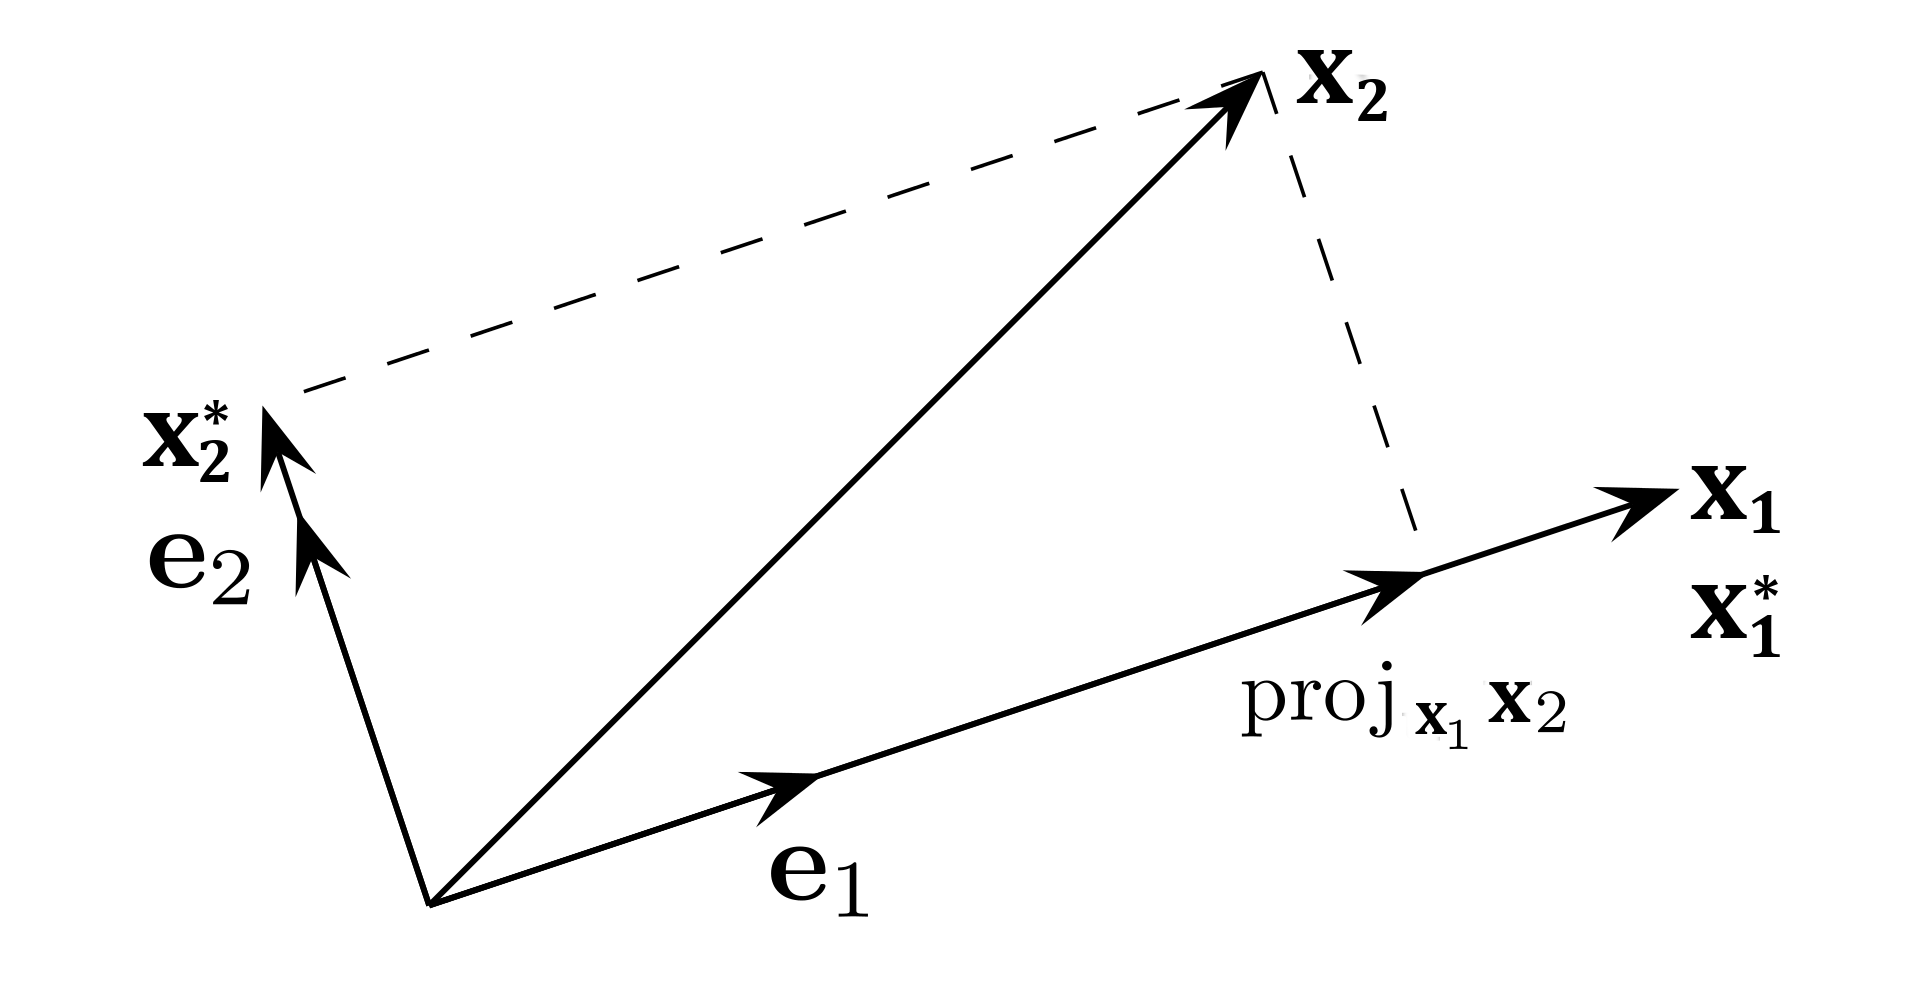
\includegraphics[scale=.7]{gs1.png}
	\caption{The first step of the Gram-Schmidt process. Image modified from \url{https://en.wikipedia.org/wiki/Gram-Schmidt_process}}
	\end{figure}
\end{frame}

\begin{frame}
	\frametitle{Gram-Schmidt}
	\begin{figure}
		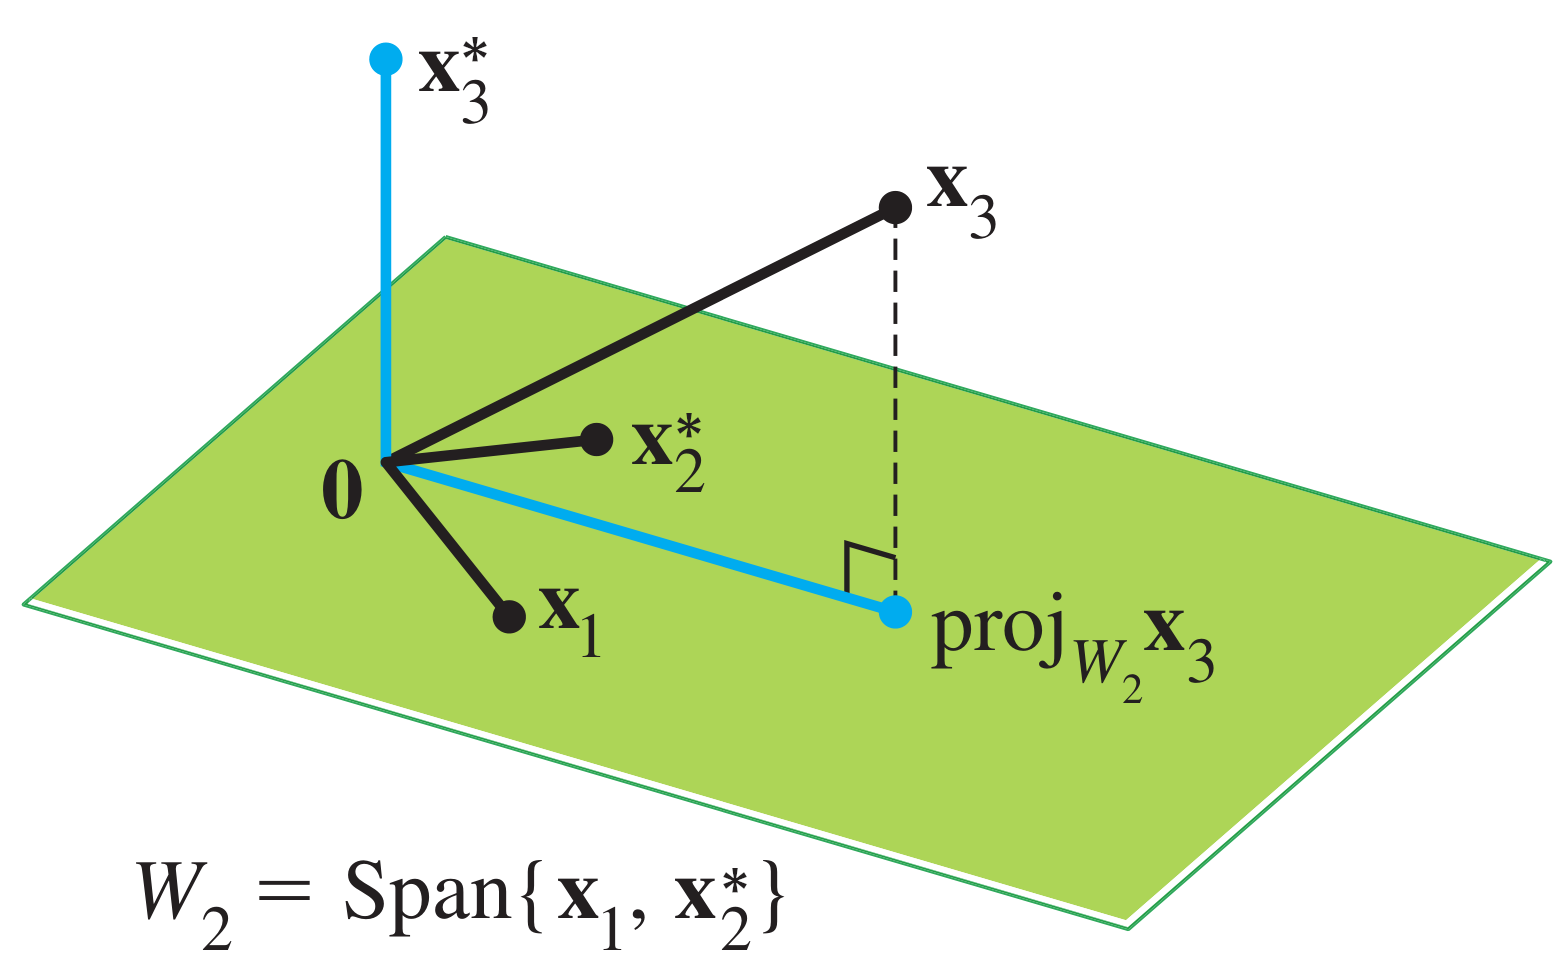
\includegraphics[scale=.2]{gs2.PNG}
		\caption{The second step of the Gram-Schmidt process. Image modified from D. Lay, S. Lay, and J. McDonald. \textit{Linear Algebra and its Applications}. Fifth Edition. 2016.}
	\end{figure}
\end{frame}

\begin{frame}
	\frametitle{A useful estimate}
	\begin{proposition}
		Let $x_1, x_2, \ldots, x_n$ be a basis for the lattice $L\subset \reals^n$ and let $x_1^*, x_2^*, \ldots, x_n^*$ be its Gram-Schmidt orthogonalization. For any nonzero $y\in L$ we have
		\[
		|y| \geq \min \{|x_1^*|, |x_2^*|, \ldots, |x_n^*|\}.
		\]
		That is, any nonzero lattice vector is at least as long as the shortest vector in the Gram-Schmidt orthogonalization.
	\end{proposition}
\end{frame}

\begin{frame}
	\frametitle{A useful estimate}
	\begin{block}{Proof}
		\begin{itemize}
			\item We can write
			\[
			y = \sum_{i=1}^nc_ix_i,\quad c_i\in \integers.\pause
			\]
			\item Since $y\neq 0$, at lease one $c_i$ is nonzero. Let $k$ be the largest index with $c_k \neq 0$.\pause
			\begin{multline*}
			y = \sum_{i=1}^k\sum_{j=1}^ic_i\mu_{ij}x_j^* = \sum_{j=1}^k\left(\sum_{i=j}^kc_i\mu_{ij}\right)x_j^*\\
			= c_kx_k^* + \sum_{j=1}^{k-1}\nu_jx_j^*,
			\end{multline*}
			for some real $\nu_j$.
		\end{itemize}
	\end{block}
\end{frame}

\begin{frame}
	\frametitle{A useful estimate}
	\begin{proof}[Proof contd...]
		\begin{itemize}
			\item Take the norm-squared on both sides.
			\begin{align*}
				|y|^2 &= \left|c_kx_k^* + \sum_{j=1}^{k-1}\nu_jx_j^*\right|^2\\
				&= c_k^2|x_k^*|^2 + \sum_{j=1}^{k-1}\nu_j^2|x_j^*|^2\\
				&\geq |x_k^*|^2\\
				&\geq \min\{|x_1^*|^2, |x_2^*|^2, \ldots, |x_n^*|^2\}.
			\end{align*}
		\end{itemize}
	\end{proof}
\end{frame}

\begin{frame}
	\frametitle{A useful equality}
	\begin{proposition}
		If $x_1, \ldots, x_n$ is a basis for the lattice $L\subset \reals^n$ and $x_1^*, \ldots, x_n^*$ is its GSO then
		\[
		\det L = \prod_{i=1}^n |x_i^*|.
		\]	
	\end{proposition}
	\begin{block}{Proof}
	\begin{itemize}
		\item We have that $\det L = \det X$, where the rows of $X$ are the basis vectors $x_1, \ldots, x_n$.
	\end{itemize}
	\end{block}
\end{frame}

\begin{frame}
	\frametitle{A useful equality}
	\begin{proof}[Proof contd...]
		\begin{itemize}
			\item By the definition of the GSO we have $X = MX^*$ where the rows of $X^*$ are the vectors $x_1^*, \ldots, x_n^*$ and $M$ consists of the GSO coefficients:
			\[
			M = \begin{bmatrix}
				1 & 0 & 0 & \cdots & 0 & 0\\
				\mu_{2,1} & 1 & 0 & \cdots & 0 & 0\\
				\mu_{3,1} & \mu_{3,2} & 1 & \cdots & 0 & 0\\
				\vdots & \vdots & \vdots & \ddots & \vdots & \vdots\\
				\mu_{n,1} & \mu_{n,2} & \mu_{n_3} & \cdots & \mu_{n,n-1} & 1
			\end{bmatrix}.\pause
			\]
			\item Since $M$ has determinant 1 we have
			\[
			\det L = |\det X| = |\det M||\det X^*| = \prod_{i=1}^n|x_i^*|.
			\]
		\end{itemize}
	\end{proof}
\end{frame}

\begin{frame}
	\frametitle{Gram-Schmidt}
	\begin{itemize}
		\item Given a basis $x_1, \ldots, x_n$ for a lattice $L\subset \reals^n$, the GSO vectors $x_1^*, \ldots, x_n^*$ need not live in $L$ since the coefficients $\frac{x_i\cdot x_j^*}{x_j^*\cdot x_j^*}$ need not be integers.\pause

		\item Can we salvage the Gram-Schmidt process and come up with a (nearly) orthogonal basis for $L$?
	\end{itemize}
\end{frame}

% \begin{frame}
% 	\frametitle{A useful equality}
% 	\begin{proof}[Proof contd...]
% 		\begin{itemize}
% 			\item Since $M$ is triangular, it has determinant 1
% 		\end{itemize}
% 	\end{proof}
% \end{frame}

\section{Basis Reduction}
%\subsection{Basis reduction}
\begin{frame}
	\frametitle{Basis reduction}
	\begin{definition}
		Let $\alpha$, $\frac{1}{4}<\alpha<1$ be a real number. Let $x_1, \ldots, x_n$ be a basis for the lattice $L\subset \reals^n$ and let $x_1^*, \ldots, x_n^*$ be its Gram-Schmidt orthogonalization. We say that the basis $x_1, \ldots, x_n$ is \textbf{$\alpha$-reduced} if
		\begin{enumerate}
			\item (size condition) $|\mu_{ij}|\leq \frac{1}{2}$ for all $i\leq j<i\leq n$,
			\item (Lov\'asz condition) $|x_i^*|^2 \geq (\alpha - \mu_{i,i-1}^2)|x_{i-1}^*|^2$ for $2\leq i \leq n$.
		\end{enumerate}
	\end{definition}
\end{frame}

\begin{frame}
	\frametitle{Size condition}
	\begin{itemize}
		\item $x_2 - \mu_{2, 1}x_1$ is orthogonal to $x_1$, but might not be in the lattice spanned by $x_1, x_2, \ldots, x_n$.\pause
		\item $x_2 - \lceil \mu_{2,1}\rfloor x_1$, where $\lceil x\rfloor$ is the integer closest to $x$ (rounded down when $x=\frac{1}{2}$), \textit{is} in the lattice and is nearly orthogonal to $x_1$.\pause
		\item The size condition, $|\mu_{ij}|\leq \frac{1}{2}$, then says that $\lceil \mu_{ij}\rfloor = 0$: $x_i$ is already nearly orthogonal to $x_j$.
	\end{itemize}
\end{frame}

\begin{frame}
	\frametitle{Lov\'asz condition}
	\begin{itemize}
		\item Assuming the size condition is met, the Lov\'asz condition, $|x_i^*|^2 \geq (\alpha - \mu_{i,i-1}^2)|x_{i-1}^*|^2$ for all $i\geq 2$, says that $x_i^*$ isn't isn't ``too much'' shorter than $x_{i-1}$.\pause
		\item Rearranging gives $|x_i^* + \mu_{i,i-1}x_{i-1}^*|^2 \geq \alpha |x_{i-1}^*|^2$. This says
		\begin{multline*}
			|\text{Projection of }x_i\text{ onto Span}\{x_1, \ldots, x_{i-2}\}|\\
			\geq \alpha|\text{Projection of }x_{i-1}\text{ onto Span}\{x_1, \ldots, x_{i-2}\}|.
		\end{multline*}
	\end{itemize}
\end{frame}

\begin{frame}
	\frametitle{Shortness}
	\begin{itemize}
		\item Let $x_1, x_2, \ldots, x_n$ be an $\alpha$-reduced basis and let $\beta = \frac{1}{\alpha - 1/4}$.\pause
		\item Combining the size and Lov\'asz conditions gives
		\[
		|x_i^*|^2 \geq (\alpha - \mu_{i,i-1}^2)|x_{i-1}^*|^2 \geq \frac{1}{\beta}|x_{i-1}^*|^2.\pause
		\]
		\item Repeatedly applying this to $x_1^* = x_1$ gives
		\[
		|x_1|^2 \leq \beta |x_2^*|^2 \leq \beta^2|x_3^*|^2 \leq \cdots \leq \beta^{n-1}|x_n^*|^2.
		\]
	\end{itemize}
\end{frame}

\begin{frame}
	\frametitle{Shortness}
	\begin{itemize}
		\item For any $2\leq i \leq n$ we have $|x_i^*|^2 \geq \beta^{-(i-1)}|x_1|^2$.\pause
		\item If we let $y$ be any nonzero vector in the lattice spanned by $x_1, \ldots, x_n$ we then have
		\[
		|y| \geq \min\{|x_1^*|, \ldots, |x_n^*|\} \geq \beta^{-(n-1)/2}|x_1|.\pause
		\]
		\item This gives a bound on the first vector in an $\alpha$-reduced basis in terms of the shortest nonzero vector $y$ in $L$:
		\[
		|x_1| \leq \beta^{(n-1)/2}|y|.
		\]
	\end{itemize}
\end{frame}

\begin{frame}
	\frametitle{Orthogonality}
	\begin{itemize}
		\item If $x_1, \ldots, x_n$ is $\alpha$-reduced, the Lov\'asz condition gives us
		\[
		|x_i^*|^2 \geq (\alpha - \mu_{i,i-1}^2)|x_{i-1}^*|^2 \geq \frac{1}{\beta}|x_{i-1}^*|^2.\pause
		\]
		\item Repeated application gives $|x_j^*|^2 \leq \beta^{i-j}|x_i^*|^2$.\pause
		\item Writing $x_i$ in terms of the GSO, $x_1^*, \ldots, x_n^*$ and applying the above inequality gives
		\[
		|x_i|^2 \leq \beta^{i-1}|x_i^*|^2.
		\]
	\end{itemize}
\end{frame}

\begin{frame}
	\frametitle{Orthogonality}
	\begin{itemize}
		\item Multiplying this inequality by itself for $1\leq i \leq n$ gives
		\[
		\prod_{i=1}^n|x_i|^2 \leq \beta^{n(n-1)/2}\prod_{i=1}^n|x_i^*|^2 = \beta^{n(n-1)/2}(\det L)^2.\pause
		\]
		\item Taking the square root and using Hadamard's inequality we have
		\[
		\det L \leq \prod_{i=1}^n|x_i| \leq \beta^{n(n-1)/4}\det L.
		\]
	\end{itemize}
\end{frame}

\section{The LLL algorithm}
\begin{frame}
	\frametitle{Can we find a reduced basis?}
	\begin{itemize}
		\item Reduced bases are nice. Their vectors are short and nearly orthogonal.\pause
		\item Does every lattice admit a reduced basis? If it does, can we compute it efficiently?
	\end{itemize}
\end{frame}

\begin{frame}
	\frametitle{The LLL algorithm}
	\begin{algorithm}[H]
	\caption{The LLL Algorithm}
	\textbf{Input: }A basis $\{x_1, \ldots, x_n\}$ of the lattice $L\subset \reals^n$ and a reduction parameter $\alpha\in (\frac{1}{4}, 1)$.\\
	\textbf{Output: }An $\alpha$-reduced basis $\{y_1, \ldots, y_n\}$ of the lattice $L$.
	\begin{algorithmic}[1]
		\State Copy $x_1, \ldots, x_n$ into $y_1, \ldots, y_n$.
		%\State Compute the GSO of $y_1, \ldots, y_n$.
		\State Set $k\gets 2$
		\While{$k\leq n$}%\Comment{Loop over the basis elements.}
			\For{$j=k-1, k-2, \ldots, 2, 1$}%\Comment{Reduce $y_k$ with the previous basis elements.}
				\State Set $y_k \gets y_k - \lceil \mu_{k,j}\rfloor y_j$.
				%\State Recompute the GSO of $y_1, \ldots, y_n$.
			\EndFor
			\If{$|y_k^*|^2 \geq (\alpha - \mu_{k,k-1}^2)|y_{k-1}^*|^2$}%\Comment{Check the Lov\'asz condition.}
				\State Set $k \gets k+1$.
			\Else
				\State Swap $y_{k-1}$ and $y_k$.
				%\State Recompute the GSO of $y_1, \ldots, y_n$.
				\State Set $k \gets \max(k-1, 2)$.
			\EndIf
		\EndWhile
		\Return $\{y_1, \ldots, y_n\}$.
	\end{algorithmic}
	\end{algorithm}
\end{frame}

\begin{frame}
	\frametitle{Why swap?}
	\begin{itemize}
		% \item The algorithm returns a reduced basis.\pause
		% \begin{itemize}
		% 	\item The loop beginning on line 4 forces the size condition.\pause
		% 	\item Checking the Lov\'asz condition on line 6 ensures that the algorithm doesn't terminate unless it is met.\pause
		% \end{itemize}
		\item If we let $L_k$ be the lattice spanned by $y_1, \ldots, y_k$, then swapping $y_k$ and $y_{k-1}$ changes the sublattices $L_k$ and $L_{k-1}$.\pause
		\item If the Lov\'asz condition isn't met then
		\[
		|y_k^*|^2 < (\alpha - \mu_{k,k-1}^2)|y_{k-1}^*|^2.\pause
		\]
		\item Since $\det L_{k-1} = |y_1^*|\cdots |y_{k-1}^*|$, replacing $y_{k-1}^*$ with the shorter $y_k^*$ will decrease $\det L_{k-1}$.\pause
		\item The swapping step attempts to order the vectors $y_i$ so that the determinants of the sublattices, $\det L_i$, are minimized.
	\end{itemize}
\end{frame}

\end{document}